\chapter{Projekt systemu Soccer Match Predictor}

\noindent Podczas projektowania systemu trzeba było podjąć decyzje na jakie komponenty powinien zostać podzielony. Ze względu na różnorodne źródła danych, pierwszym krokiem było połączenie ich w jeden spójny zbiór. W tym celu powstała baza danych Microsoft SQL Server, która jest dostępna na platformie Azure Cloud dla każdego potencjalnego użytkownika. Baza jest przeniesiona z bazy danych SQLite \cite{kagggle_european_soccer_database}, ale musiała zostać uzupełniona innymi źródłami danych. W tym celu utworzona została konfigurowalna aplikacja konsolowa.

Kolejną decyzją do podjęcia był transfer danych z przygotowanego źródła, do skryptów przygotowujących cechy dla algorytmów uczenia maszynowego. Komponentem do tego wykorzystywanym jest aplikacja internetowa, utworzona jako WebAPI. Założone zostało, że zapytania do bazy danych powinny zostać wykonane na niezależnym poziomie, aby umożliwić wykorzystanie zasobów platformy Azure Cloud.

W celu rozdzielenia algorytmów i przygotowywania cech, które otrzymają one na wejściu, powstała biblioteka w utworzona w języku Python. dzięki temu twórcy algorytmów uczących mogą niezależnie otrzymywać jednolicie przetworzone dane.

Wszystkie te komponenty są zapleczem dla głównego celu systemu, czyli środowiska w którym użytkownik będzie mógł skorzystać z wcześniej przygotowanych danych i algorytmów. Jest nim Interaktywny \textit{Jupter Notebook}, który jest narzędziem do wykonywania predykcji przez utworzone algorytmy.

Cały system przedstawia schemat widoczny na rysunku \ref{fig:arch1}.
\newpage

\section{Ogólny schemat systemu i jego architektura}
\label{arch}
    \begin{figure}[h] 
        \centering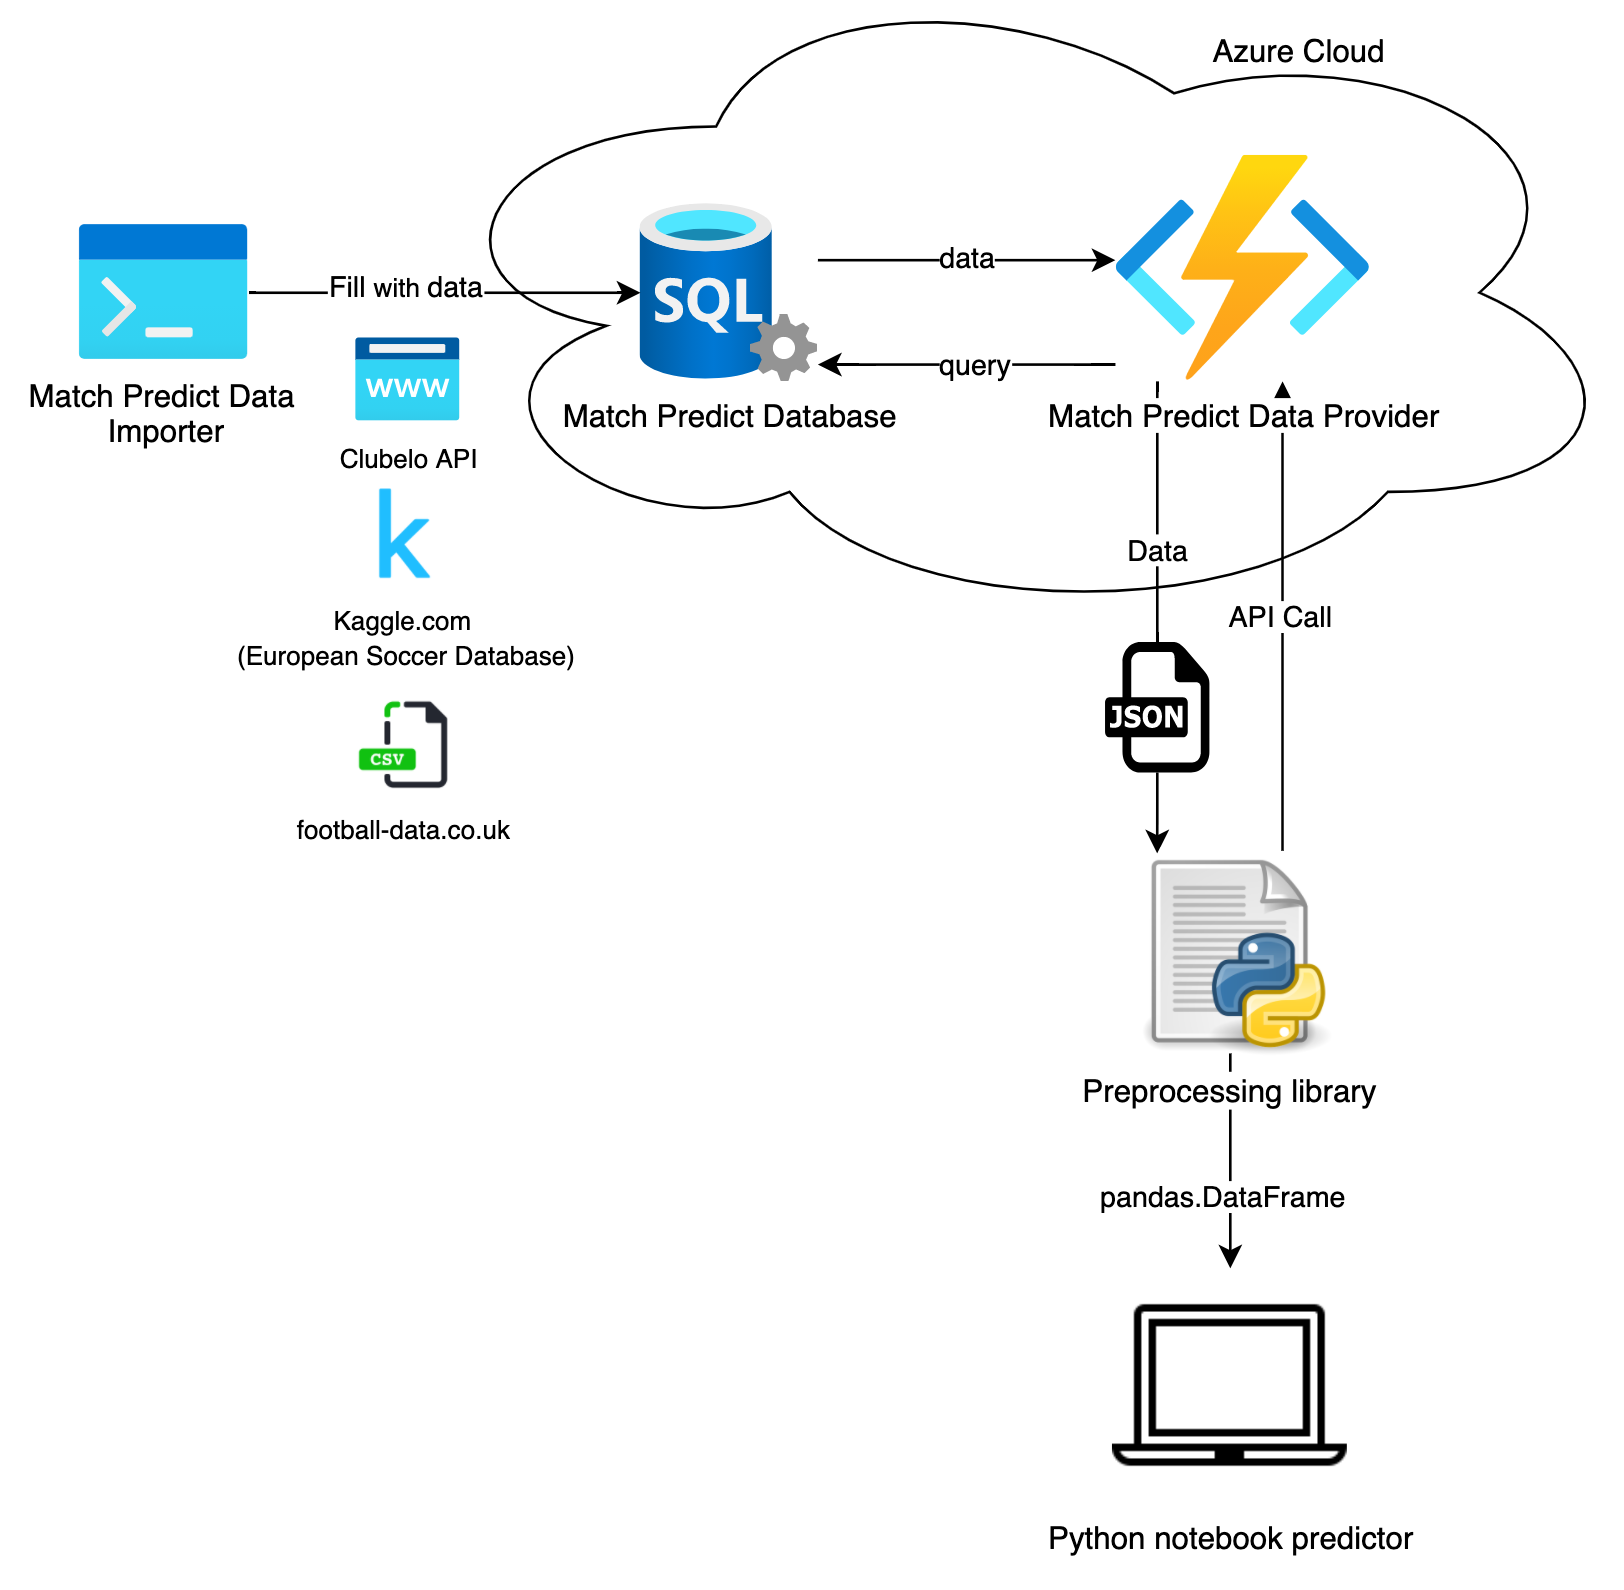
\includegraphics[width=\textwidth]{figures/MatchPredictorArchitecture.png}
        \caption{Architektura systemu Soccer Match Predictor}
        \label{fig:arch1}
    \end{figure}
\newpage

\noindent Pierwszym komponentem jest \textbf{Match Predict Data Importer}, dalej nazywany \definicja{MPDI}. Jest to aplikacja konsolowa napisana w języku C\#, której zadaniem jest import danych z różnych źródeł do docelowej bazy danych widocznej na schemacie jako \textbf{Match Predict Database}.

Baza jest przechowywanym na chmurze Azure komponentem Microsoft SQL Server, w której przechowywane są wszelkie dane wykorzystywane dalej w systemie. Schemat bazy danych jest przedstawiony w sekcji \ref{database_schema}.

Match Predict Data Provider (dalej zwany \definicja{MPDP}) służy w produkcie jako WebAPI, które przesyła dane w formacie JSON. Dane pochodzą z bazy Match Predict Database i są odpowiednio agregowane. Komponent ten to aplikacja Azure Function napisana w języku C\#, która znajduje się na chmurze Azure.

~

Kolejnym komponentem w systemie widocznym na schemacie jako \textbf{Preprocessing library} jest biblioteka służąca do pobierania danych i ich wstępnego przetwarzania wraz z tworzeniem zbioru cech. Jest to moduł napisany w języku Python, który może być wykorzystany w dowolnej aplikacji napisanej w tym języku. Komunikuje się on z opisaną wyżej bazą danych przy pomocy udostępnionego przez nią interfejsu WebAPI i otrzymuje od niego dane w formacie JSON, natomiast korzystającym z niego klientom przekazuje wygodne do operowania dane w formacie \definicja{pandas.DataFrame}. 

Uniwersalność tego modułu polega na tym, że całkowicie chowa on szczegóły implementacji swoich operacji pobierania danych z bazy, przetwarzania ich i tworzenia cech i udostępnia jedynie metody pozwalające na pobranie danych dla konkretnych sezonów i/lub konkretnych drużyn. Dzięki temu klient korzystający z tego modułu jest niezależny od wszelkich zmian strukturalnych w bazie danych czy interfejsie służącym do komunikacji z nią.

~

Ostatnim elementem jest widoczny na schemacie \textbf{Python notebook predictor}, który służy jako środowisko testowe do porównywania różnego rodzaju algorytmów stosując różne podejścia i techniki. Jest to aplikacja stworzona w \textit{Jupter Notebook}, czyli rozbudowanym narzędziu uruchamianym w przeglądarce internetowej pozwalającym na m.in. separowanie poszczególnych części kodu i uruchamianie ich niezależnie od siebie. Pozwala to na przykład na jednorazowe pobranie danych na samym początku i wielokrotne użycie ich w późniejszych eksperymentach.

Środowisko to jest klientem opisanego wyżej modułu do wstępnego przetwarzania danych i korzysta z niego do pobierania przetworzonych danych. 

\newpage
\section{Schemat bazy danych}
\label{database_schema}
\begin{figure}[h]
  \centering
   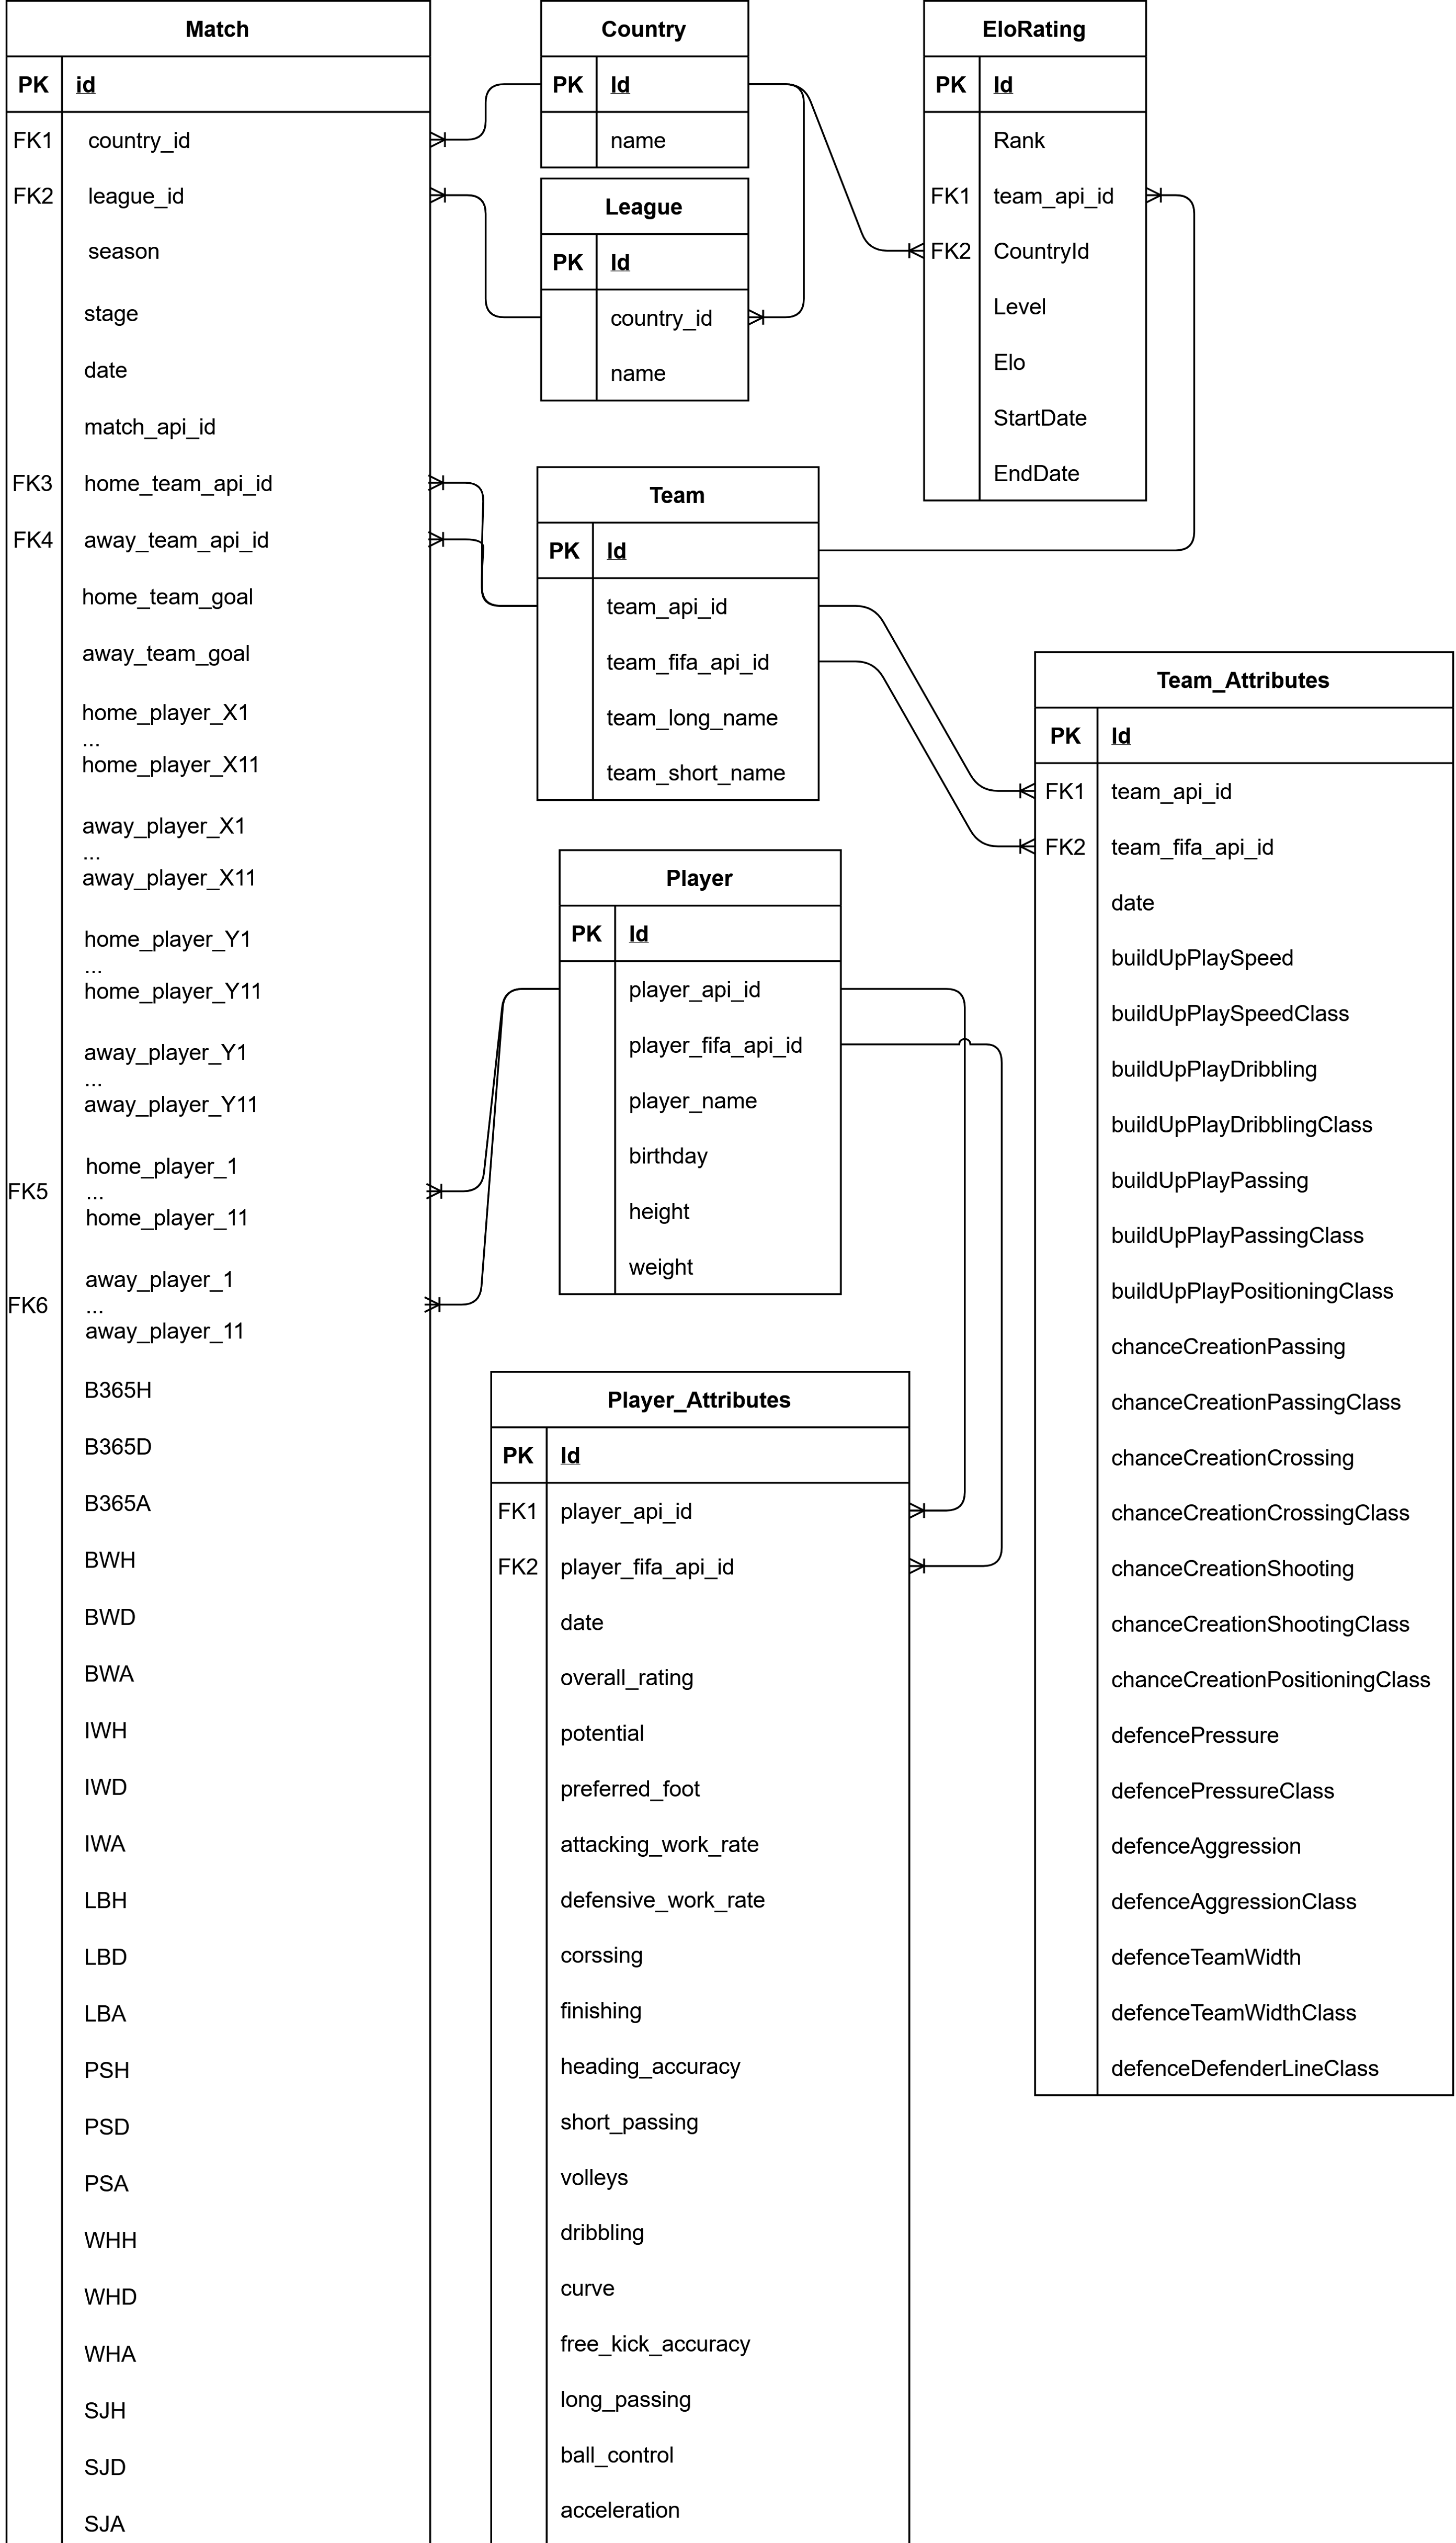
\includegraphics[width=0.83\textwidth]{figures/match_predict_schema_1.png}%

\end{figure}
\newpage
\begin{figure}[h]
\ContinuedFloat
    \centering
  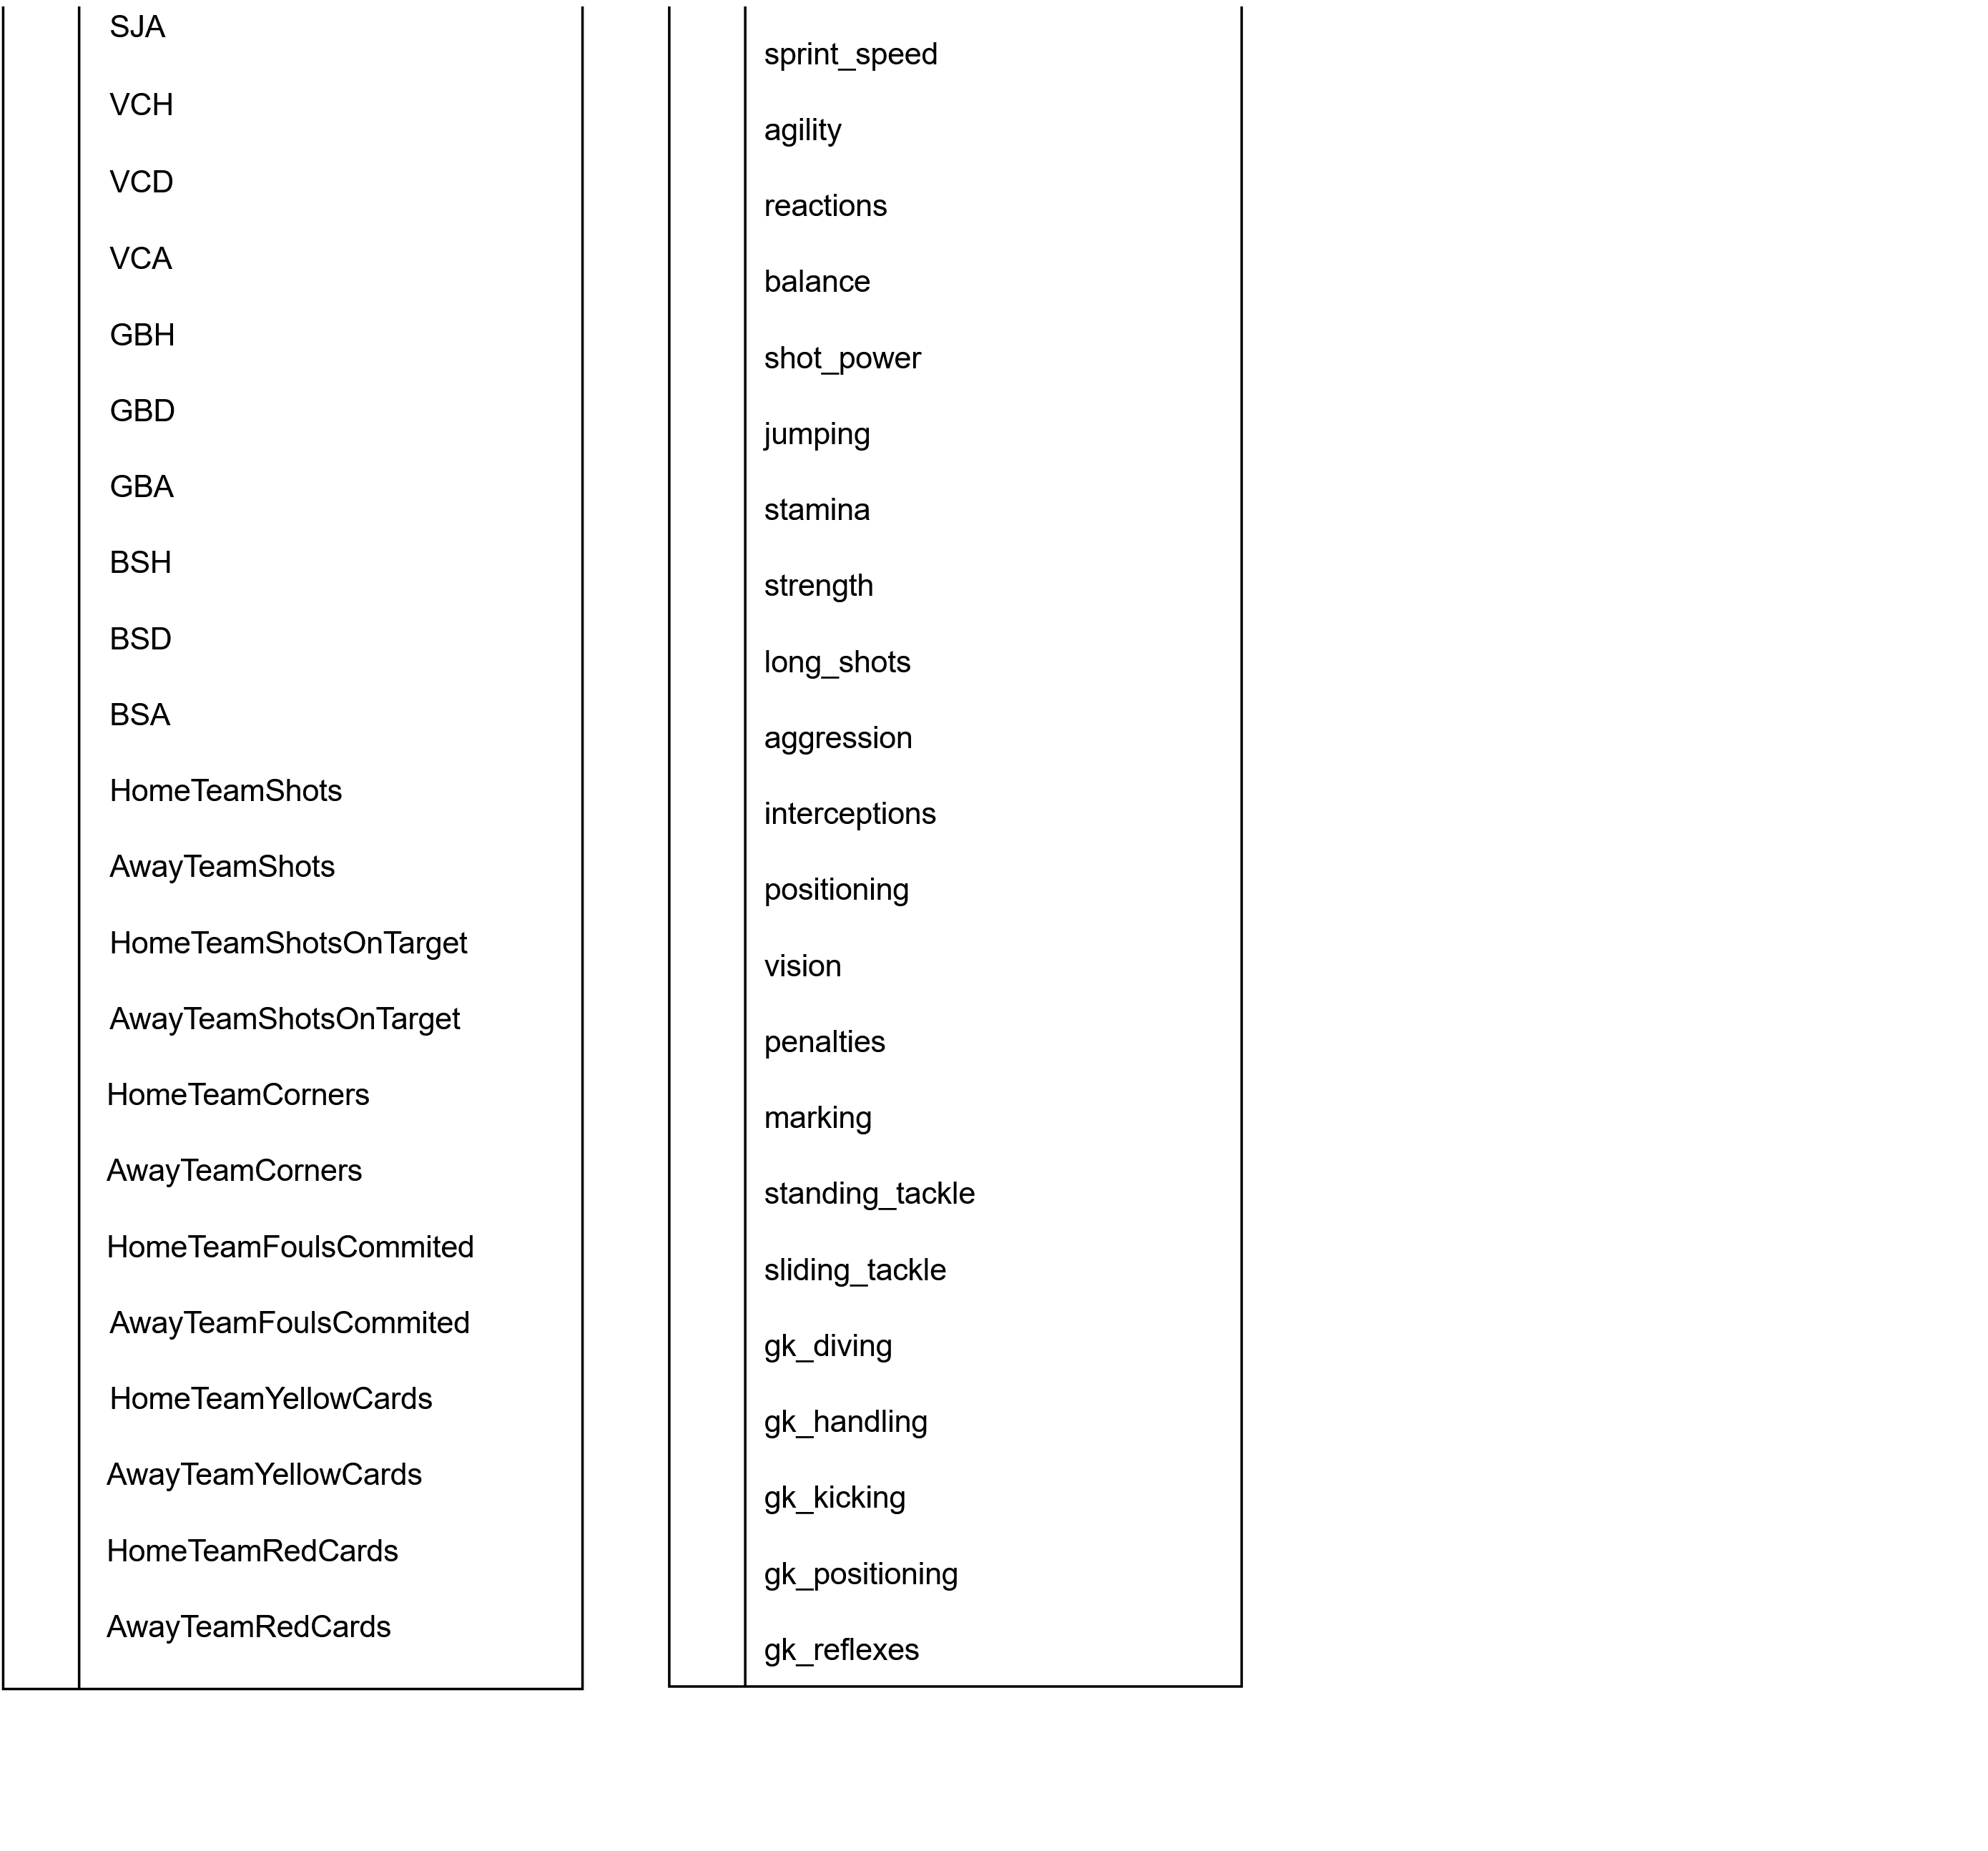
\includegraphics[width=0.83\textwidth]{figures/match_predict_schema_2.png}%
  \addtocounter{figure}{1}
  \caption{Schemat bazy danych \textit{Match Predict}}
    
  \label{fig:match_predict_schema}
    
\end{figure}
 
\noindent Rysunek \ref{fig:match_predict_schema} przedstawia schemat bazy danych \textit{Match Predict Database} widocznej na rysunku architektury systemu \ref{fig:arch1}. Jest to relacyjna baza danych, stworzona jak to wcześniej wspomniane w \ref{arch}, przy użyciu technologii Microsoft SQL Server.

Bazą dla schematu była pozyskana z strony Kaggle.com baza \textit{European Soccer Database} \cite{kagggle_european_soccer_database}. Została przerobiona, aby działała w systemie Microsoft SQL Sever i odpowiednio przefiltrowana, tak aby zawierała dane tylko z interesującej nas ligi angielskiej.

W centrum wszystkich tabel znajduję się tabela \textbf{Match}. Zawiera on dane dotyczące poszczególnych meczy, które zostały zagrane w latach 2008-2016 w lidze angielskiej. Gdzie: 
\begin{itemize}
    \item Id jest kluczem głównym tabeli, unikatowym identyfikatorem meczu.
    
    \item Pola country\_id oraz league\_id są kluczami obcymi do odpowiednie tabel \textbf{Country} oraz \textbf{League}.
    
    \item Season oznacza w jakim sezonie został zagrany mecz, zapisane w formacie \{rok\}/\{rok+1\}.
    
    \item Stage oznacza numer kolejki ligowej
    
    \item Date to data zagranego meczu.
    
    \item Match\_api\_id również jest unikatowym identyfikatorem, znajduję się on w bazie jako id pochodzące z źródłowego zbioru danych         \cite{football_data_enetscore}.
    
    \item Home/away\_team\_api\_id to klucze obce wskazujące na tabele \textbf{Team}. Odnoszą się one do api\_id, które po raz kolejny są       unikalnym identyfikatorem drużyn z oryginalnego źródła danych.
    
    \item Home/away\_team\_goal to liczba goli strzelonych przez poszczególne drużyny w trakcie meczu
    
    \item Pola home/away\_player\_X1-11 oraz home/away\_player\_Y1-11 oznaczają pozycje zawodnika na boisku.
    
    \item Pola home/away\_player\_1-11 są kluczami obcymi, które odnoszą się do tabeli \textbf{Player}. Zawierają wartości player\_api\_id poszczególnych zawodników biorących udział w rozgrywce.
    
    \item Widoczne na schemacie \ref{fig:match_predict_schema} pola zaczynając od B365H do BSA to wartości przedstawiające wysokości kursów, które poszczególne zakłady bukmacherskie na dany moment przyjmowały zakłady. Kolumny kończące się na H wskazują zakład oznaczający wygraną gospodarza, kończące się na 'A' wygraną drużyny gości, a 'D' oznacza kurs na zakłady, które oznaczają remis. Według opisu zbioru danych z strony Kaggle.com \cite{kagggle_european_soccer_database}, dane te pochodzą z strony www.football-data.co.uk, gdzie można znaleźć historyczne wartości zakładów bukmacherskich w lidze angielskiej.
    
    \item Pola od HomeTeamShots do AwayTeamRedCard w tabeli \textbf{Match} zawierają wszelkie statystyki meczu takie jak strzały na bramkę, faule, ilości żółtych i czerwonych kartek w meczu.
\end{itemize}

Tabele \textbf{Country} oraz \textbf{League} zawierają tylko informacje o nazwach kolejno kraju oraz ligi. Obecna zawartość tych tabel to pojedyncze wpisy, jednak pozostały w bazie w razie dalszego rozwoju projektu.

Encja \textbf{Team} zawiera nazwy drużyn oraz ich identyfikatory z oryginalnych źródeł danych (team\_api\_id \cite{football_data_enetscore} oraz team\_fifa\_api\_id \cite{Sofifa}).

Tabela \textbf{Team\_Attributes} jest wypełniona informacjami o statystykach drużyny, które zostały zebrane z corocznych wydań gry Fifa produkowanej przez firmę E.A Games. Autor zestawu danych z strony Kaggle.com \cite{kagggle_european_soccer_database} zdobył te dane z strony internetowej zawierającej te statystyki \cite{Sofifa}. Każdy wpis w encji zawiera datę, dzięki której wiemy do którego roku odnosi się danych wpis dla danej drużyny. Klucze obce team\_api\_id oraz team\_fifa\_api\_id są referencją do tabeli \textbf{Team}.

Encja \textbf{Player} posiada podstawowe informacje o poszczególnych zawodnikach takie jak wzrost, rok urodzenia i wagę. Oprócz podobnie jak w tabeli \textbf{Team} posiada unikalne identyfikatory, które pochodzą z oryginalnych źródeł.

Podobnie jak w przypadku drużyn, każdy zawodnik posiada zestaw statystyk określających jego poziom w odpowiedniej tabeli o nazwie \textbf{Player\_Attributes}. Zawartość tej encji również została zebrana z strony internetowej, która posiada informacje o zawodnikach w corocznych wydania gry Fifa \cite{Sofifa}. Tak samo również posiada datę, określającą rok dla którego te dane są aktualne. Klucze obce player\_api\_id oraz player\_fifa\_api\_id są referencją do tabeli \textbf{Player}. 

Ostatnią tabelą która znajduje się na schemacie \ref{fig:match_predict_schema} jest \textbf{EloRating}. Dane w tej tabeli pochodzą z strony internetowej \url{http://clubelo.com/} a główną wartością pobieraną z niej to wartość Elo. \definicja{StartDate} oraz \definicja{EndDate} to towarzyszące tej wartości momenty, między którymi była obowiązująca. Rank to miejsce w rankingu danej drużyny, gdzie kryterium jest właśnie 'Elo rating'. Team\_api\_id to klucz obcy odnoszący się do tabeli \textbf{Team}, służący do ustalenia, do której drużyny należy dany wpis Elo. CountryId to klucz obcy do encji \textbf{Country}.

Wszystkie tabele mają klucz główny oznaczony jako Id, który jest unikalną liczbą identyfikującą jednoznacznie każdy wpis w poszczególnych tabelach.

\section{Opis web API}
\section{Środowisko użytkownika docelowego}
\noindent
Jak wspomniano wcześniej, aplikacja jest tworzona dla osób chętnych wzięcia udziału w zakładach bukmacherskich oraz analityków i statystyków konkretnych drużyn, które posiadałyby chęć sprawdzenia aktualnej formy swojego zespołu i porównania z innym zespołem i na podstawie tego oraz otrzymanego przewidywanego wyniku określić taktykę na nadchodzący mecz. Wiele osób pożąda takich informacji ponieważ są one odpowiedzią zwrotną otrzymywaną nie w czasie lub po rozegranym meczu, lecz przed nim. Dzięki posiadaniu takich informacji można dobrać odpowiednią taktykę, zmienić skład wyjściowy danego zespołu czy zastosować jeszcze inne modyfikacje w celu maksymalizacji szansy na wygraną. Jednak jak powszechnie wiadomo, nie każdy posiada zdolności programistyczne. Jednak analitycy sportowi jak i osoby interesujące się szeroko pojętą informatyką, będą potrafiły skorzystać z przygotowanego środowiska do pozyskiwania odpowiedzi zbudowanego systemu dla konkretnych zapytań. Nie jest tu potrzebna zdolność programistyczna, a jedynie wymagana jest wiedza jak załadować i otworzyć dany interfejs (jeśli potencjalny użytkownik nie wyrazi chęci instalacji \definicja{jupter notebook} na swoim komputerze, istnieje wiele różnych środowisk internetowy, które można bezpłatnie wykorzystywać, w tym ładować odpowiednie pliki i uruchamiać dane skrypty. Jednym z nich jest popularna platforma chmurowa \definicja{Google colab}). 

Interfejs użytkownika przedstawia się w następujący sposób:
\begin{figure}[H] 
        \centering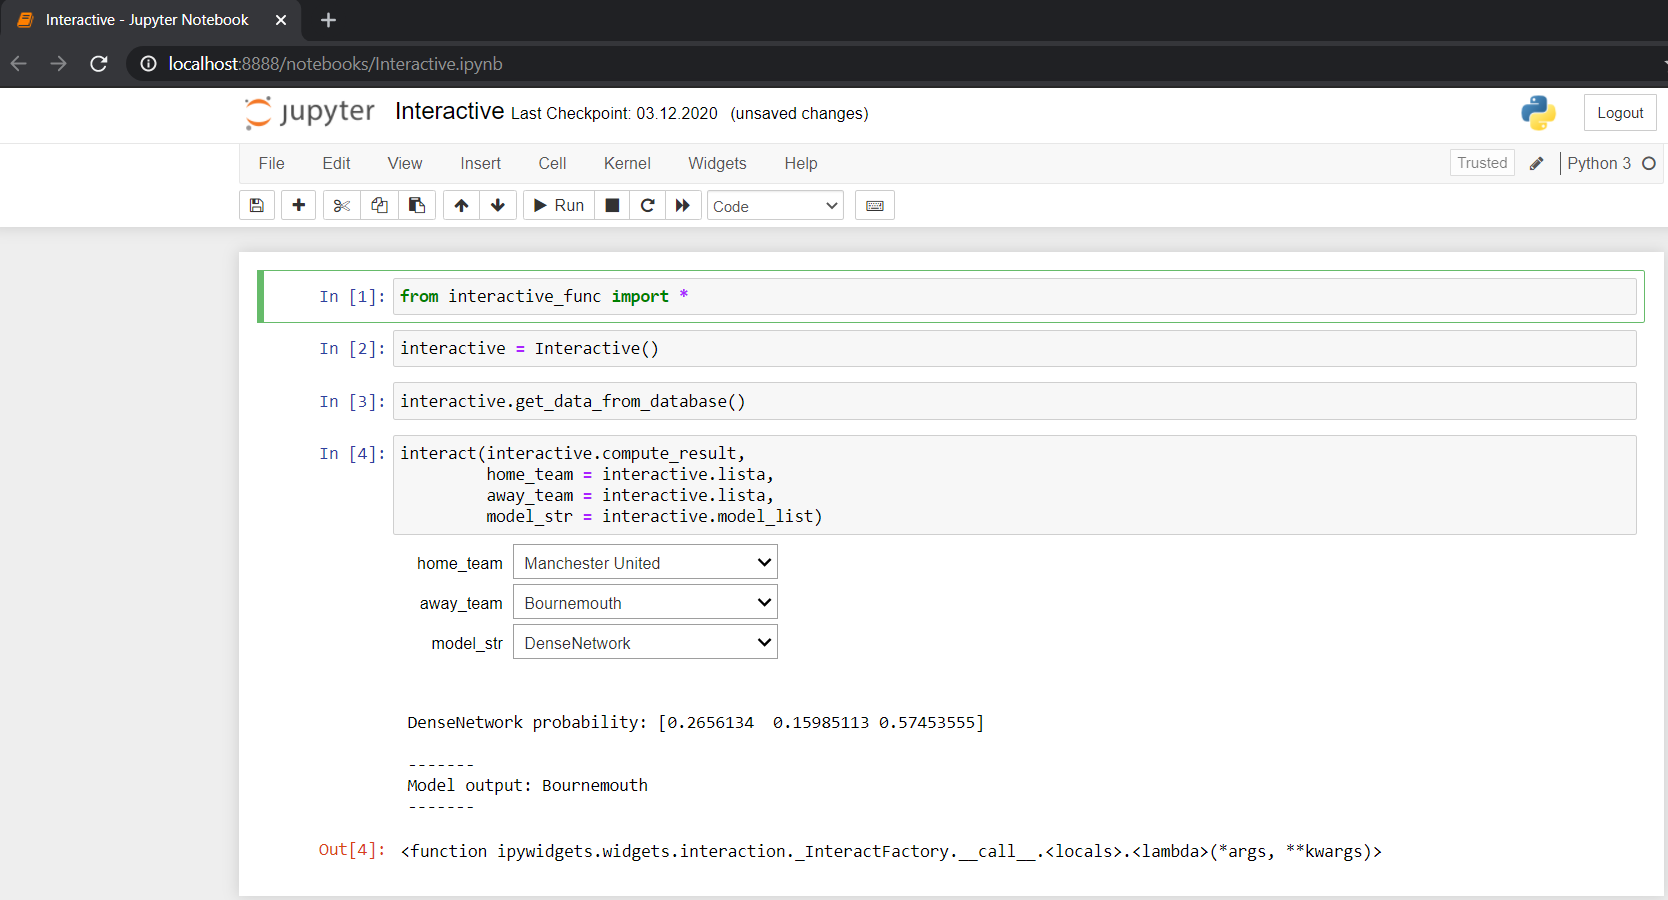
\includegraphics[width=16cm,height=10cm]{figures/Interactive_overview.png}
        \caption{Interaktywny notebook}\label{interactive}
\end{figure}
Do uruchomienia środowiska potrzebne jest uruchomienie czterech przedstawionych powyżej komórek programu, a funkcje, które zostaną dzięki temu wykonane, zadbają o to by użytkownik mógł bez pisania jakiegokolwiek kodu pobrać wymagane dane a następnie dokonać predykcji.

Wybór drużyn odbywa się poprzez wybór z rozwijanego menu:
\begin{figure}[H] 
        \centering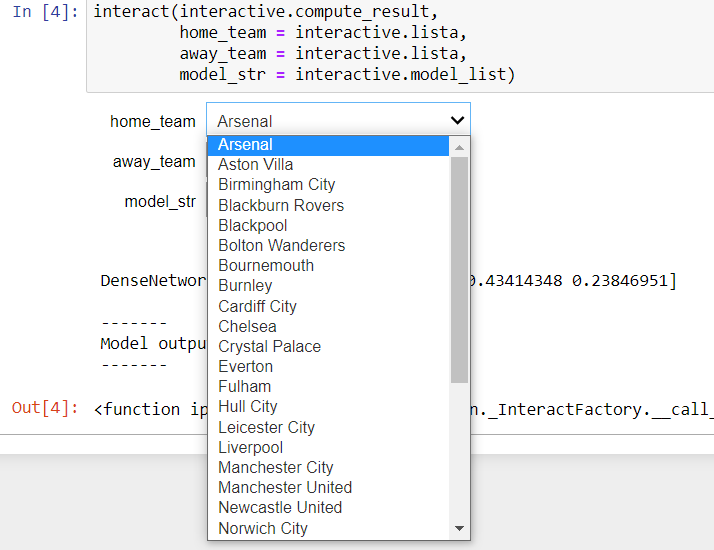
\includegraphics[width=10cm,height=8cm]{figures/Interactive_team_selection.png}
        \caption{Interaktywny wybór drużyn}\label{interactive_tem}
\end{figure}
Dodatkowo, pozwala się użytkownikowi na wybór preferowanego przez niego algorytmu, za pomocą którego zwrócony zostanie wynik predykcji:
\begin{figure}[H] 
        \centering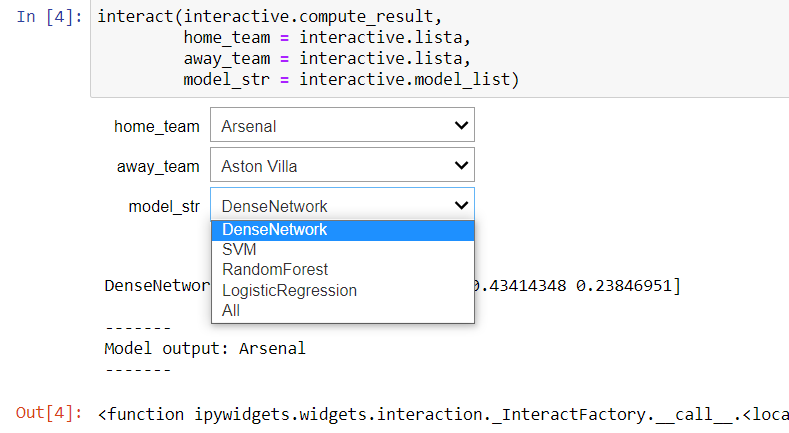
\includegraphics[width=12cm,height=8cm]{figures/Interactive_alg_selection.png}
        \caption{Interaktywny wybór algorytmu}\label{interactive_alg}
\end{figure}
W momencie, kiedy użytkownik wyraziłby chęć wykorzystania wszystkich algorytmów, zostaje mu udostępniona taka możliwość i na zasadzie głosowania większościowego (klasa, które uzyska większość głosów zostaje zwrócona, w przeciwnym wypadku komunikat od braku dominanta i zachęcenia do wybrania konkretnego algorytmu) użytkownik jest wstanie uzyskać wynik. W przypadku algorytmów, które zwracają rozkład prawdopodobieństwa przynależności do konkretnych klas wynikowych, również ta informacja jest zwrócona i wyświetlona dla użytkownika, w celu pokazania mu czy dany wynik jest bardziej lub mniej pewny według wybranego algorytmu. 

\begin{figure}%
    \centering
    \subfloat[\centering Wynik wraz z prawdopodobieństwem]{{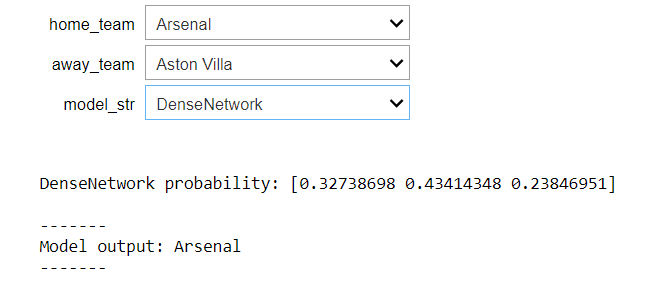
\includegraphics[width=6cm,height=5cm]{figures/Interactive_results.png} }}%
    \qquad
    \subfloat[\centering Brak wyniku dominującego]{{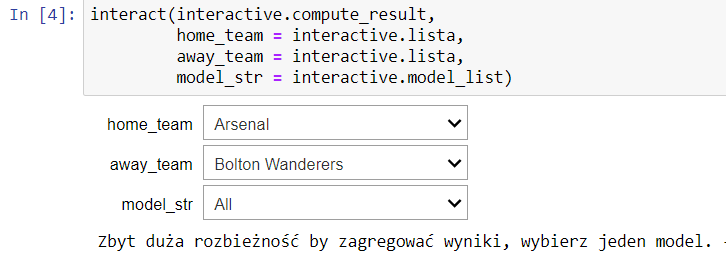
\includegraphics[width=8cm,height=5cm]{figures/Interactive_results2.png} }}%
    \caption{Otrzymywane odpowiedzi zwrotne}%
    \label{fig:Results}%
\end{figure}
Tak więc, interaktywny notebook jest bardzo prostym lecz zarazem intuicyjnym interfejsem, który każdy może z powodzeniem wykorzystać i odczytać wyniki na podstawie nauczonych przez nas modeli predykcyjnych.
\section{Ew. dodatkowe narzędzia analizy danych}